\documentclass[12pt]{article}
\usepackage[utf8]{inputenc}
\usepackage{amsmath}
\usepackage{listings}
\usepackage{graphicx}
\usepackage{fancyhdr}

\title{Introduction to Model-based AI Coursework 2}
\author{Miki Ivanovic}
\date{March 2019}

\begin{document}

\maketitle
	

\section{}

\begin{figure}[ht!]
\centering
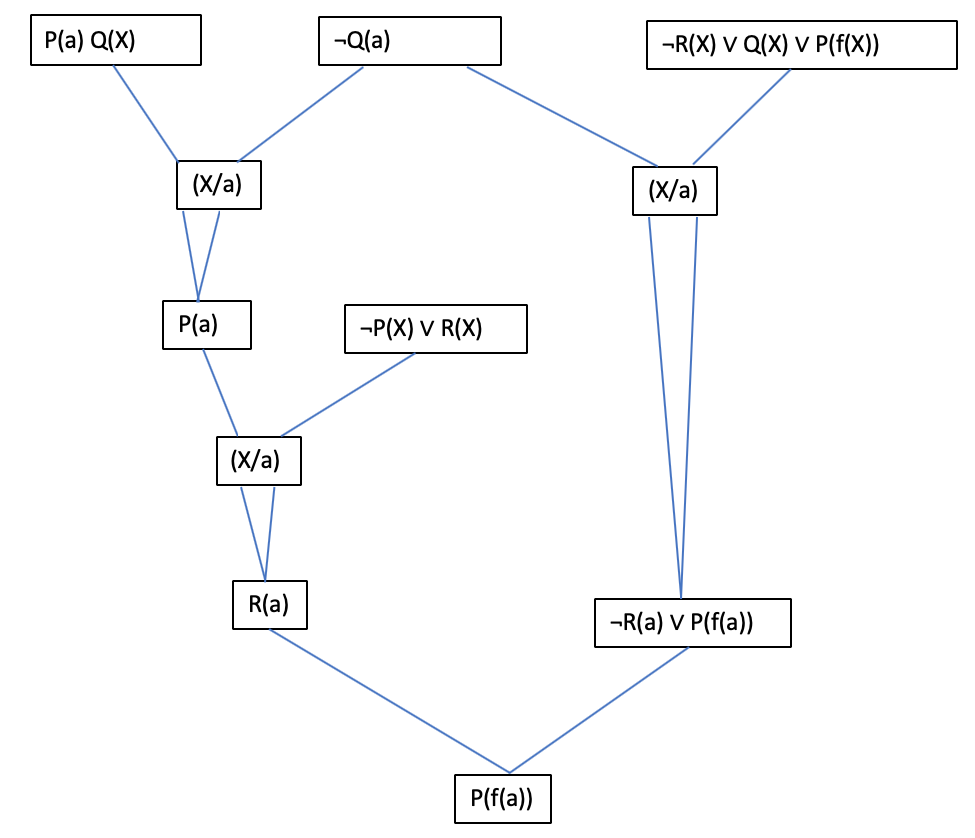
\includegraphics[width=90mm]{part1.png}
\end{figure}

\section{}

There are two constants $a$ and $c$ and no function definitions within $S$, therefore we generate a ground instance $S'$ of $S$

$$
ground(S) = S' = \{ G(c), B(a), G(a) \lor\neg G(c), \neg B(a) \lor\neg G(a)\}
$$ 

$S'$ is a finite set of ground instances which is clearly unsatisfiable, therefore by the Herbrand Theorem we have $S$ is unsatisfiable $\Rightarrow S$ has no valid Herbrand interpretations.

\section{}

Let 
\begin{align*}
ground(S) = S' = 
\{&
\neg P(a,a) \lor P(a,a),\neg P(a,b) \lor P(a,b),\neg P(b,a) \lor P(a,a),
\\& \neg P(b,b) \lor P(a,b),
P(a,a) \lor P(b,a), P(a,b) \lor P(b,b),
\\&\neg P(a,b) \lor \neg P(a,a), \neg P(a,b) \lor \neg P(b,b)
\}
\end{align*}

\begin{itemize}

\item Basic Davis Putnam

Remove tautologies

\begin{align*}
S'_1 = \{ &
\neg P(b,a) \lor P(a,a), \neg P(b,b) \lor P(a,b),
P(a,a) \lor P(b,a), \\&
P(a,b) \lor P(b,b),
\neg P(a,b) \lor \neg P(a,a), \neg P(a,b) \lor \neg P(b,b)
\}
\end{align*}

choose $P(a,a)$

\begin{align*}
S'_2 = \{ &
\neg P(b,b) \lor P(a,b),
P(a,b) \lor P(b,b),
\neg P(a,b) \lor \neg P(b,b),
\\&\neg P(b,a) \lor \neg P(a,b), 
\neg P(b,a) \lor \neg P(a,b)
\}
\end{align*}

choose $P(a,b)$

\begin{align*}
S'_3= \{&
\neg P(b,b), \neg P(b,b)\lor \neg P(b,a), 
\neg P(b,a) \lor P(b,b), P(b,b) \lor \neg P(b,a)
\}
\end{align*}

choose $P(b,a)$

\begin{align*}
S'_4= \{&
\neg P(b,b), P(b,b)
\}
\end{align*}

choose $P(b,b)$

$$
S'_5 = \{ \{ \} \}
$$

\item DLL

\begin{figure}[ht!]
\centering
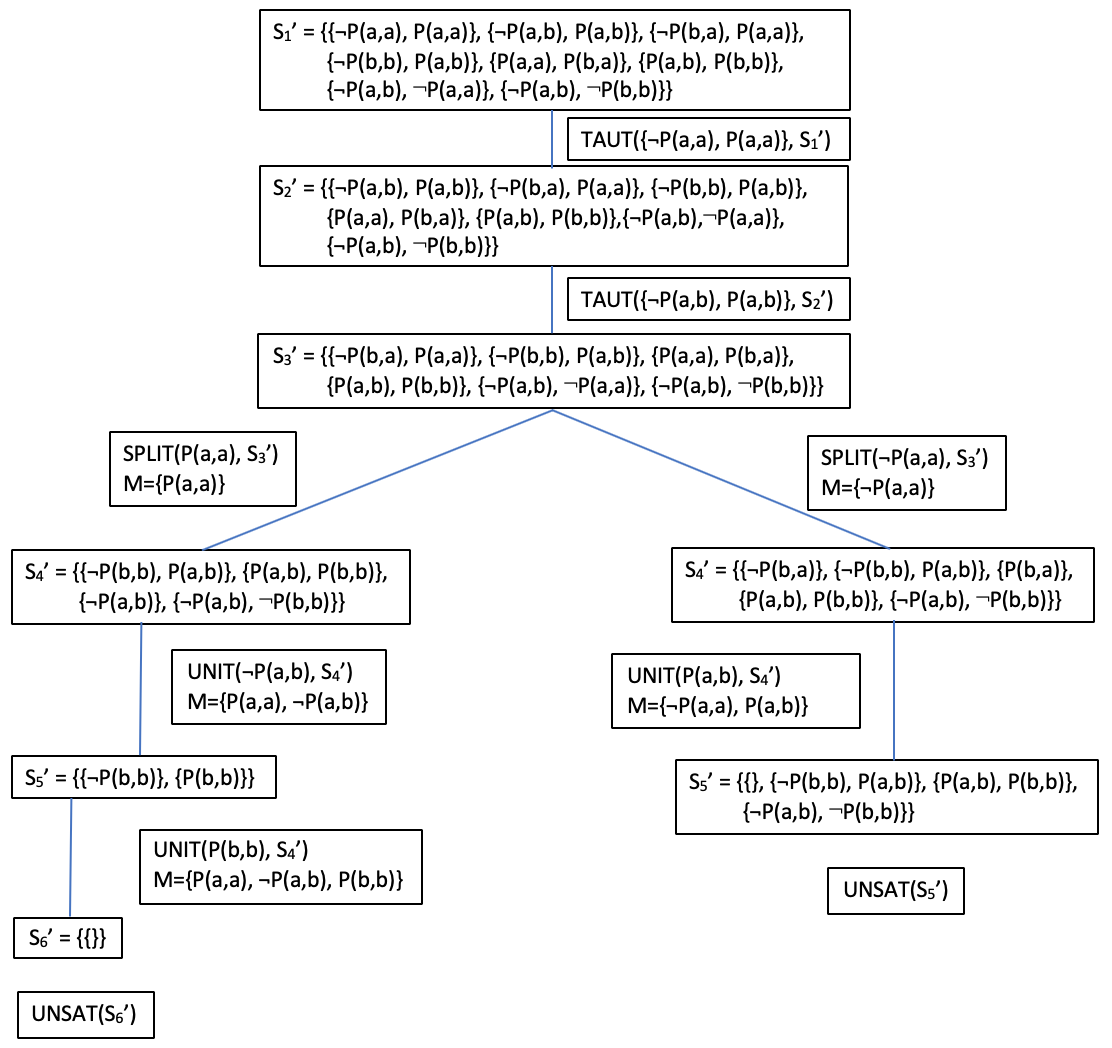
\includegraphics[width=90mm]{part3b.png}
\end{figure}

\end{itemize}

\section{}

\subsection{}

\begin{lstlisting}

%static facts:
place(house)
place(car)

%initially we have
%	agent in house
%	camera in car
%	camera switched off

initially(agentLocation(house))
initially(cameraLocation(car))
initially(cameraStatus(off))

%describe agent taking picture
initiates(takePhoto,photoTaken(Place),T) :-
	time(T),
	holds(holdCamera, T),
	holds(agentLocation(Place,T).

%describe agent turning on camera
initiates(turnOn,cameraStatus(on),T) :-
	time(T),
	holds(holdCamera,T),
	holds(cameraStatus(off),T).

terminates(turnOn,cameraStatus(off),T) :-
	time(T),
	holds(holdCamera,T),
	holds(cameraStatus(off),T).

%describe picking up camera
initiate(pickUp,holdCamera,T) :-
	time(T),
	holds(not holdCamera,T),
	holds(agentLocation(Place1),T),
	holds(cameraLocation(Place2),T),
	Place1 == Place2.

%describe agent moving location
initiates(go(P1,P2),agentLocation(P2),T) :-
	place(P1),
	place(P2),
	P1 =/= P2,
	time(T).					

terminates(go(P1,P2),agentLocation(P1),T) :-
	place(P1),
	place(P2),
	P1 =/= P2,
	time(T).					

%describe putting down camera
initiate(putDown, not holdCamera,T) :-
	time(T),
	holdAt(holdCamera, T).

%describe agent turning off camera
initiates(turnOff,cameraStatus(off),T) :-
	time(T),
	holds(holdCamera,T),
	holds(cameraStatus(on),T).

terminates(turnOff,cameraStatus(on),T) :-
	time(T),
	holds(holdCamera,T),
	holds(cameraStatus(on),T).
	

%only one event can happen at a given time
ic :- happens(E1,T), happens(E2,T), time(T), E1 =/= E2.


abducible(happens(_,_)).


%Goal: take photo of house
holds(photoTaken(house),_)

\end{lstlisting}

\subsection{}

$
\Delta =
$

\begin{lstlisting}
{happens(go(house,car),1), happens(pickUp,2),
 happens(turnOn,3), happens(go(car,house),4),
 happens(takePhoto,5)}
\end{lstlisting}

\subsection{}

\end{document}
